% Options for packages loaded elsewhere
\PassOptionsToPackage{unicode}{hyperref}
\PassOptionsToPackage{hyphens}{url}
%
\documentclass[
  man]{apa6}
\usepackage{amsmath,amssymb}
\usepackage{lmodern}
\usepackage{iftex}
\ifPDFTeX
  \usepackage[T1]{fontenc}
  \usepackage[utf8]{inputenc}
  \usepackage{textcomp} % provide euro and other symbols
\else % if luatex or xetex
  \usepackage{unicode-math}
  \defaultfontfeatures{Scale=MatchLowercase}
  \defaultfontfeatures[\rmfamily]{Ligatures=TeX,Scale=1}
\fi
% Use upquote if available, for straight quotes in verbatim environments
\IfFileExists{upquote.sty}{\usepackage{upquote}}{}
\IfFileExists{microtype.sty}{% use microtype if available
  \usepackage[]{microtype}
  \UseMicrotypeSet[protrusion]{basicmath} % disable protrusion for tt fonts
}{}
\makeatletter
\@ifundefined{KOMAClassName}{% if non-KOMA class
  \IfFileExists{parskip.sty}{%
    \usepackage{parskip}
  }{% else
    \setlength{\parindent}{0pt}
    \setlength{\parskip}{6pt plus 2pt minus 1pt}}
}{% if KOMA class
  \KOMAoptions{parskip=half}}
\makeatother
\usepackage{xcolor}
\usepackage{graphicx}
\makeatletter
\def\maxwidth{\ifdim\Gin@nat@width>\linewidth\linewidth\else\Gin@nat@width\fi}
\def\maxheight{\ifdim\Gin@nat@height>\textheight\textheight\else\Gin@nat@height\fi}
\makeatother
% Scale images if necessary, so that they will not overflow the page
% margins by default, and it is still possible to overwrite the defaults
% using explicit options in \includegraphics[width, height, ...]{}
\setkeys{Gin}{width=\maxwidth,height=\maxheight,keepaspectratio}
% Set default figure placement to htbp
\makeatletter
\def\fps@figure{htbp}
\makeatother
\setlength{\emergencystretch}{3em} % prevent overfull lines
\providecommand{\tightlist}{%
  \setlength{\itemsep}{0pt}\setlength{\parskip}{0pt}}
\setcounter{secnumdepth}{-\maxdimen} % remove section numbering
% Make \paragraph and \subparagraph free-standing
\ifx\paragraph\undefined\else
  \let\oldparagraph\paragraph
  \renewcommand{\paragraph}[1]{\oldparagraph{#1}\mbox{}}
\fi
\ifx\subparagraph\undefined\else
  \let\oldsubparagraph\subparagraph
  \renewcommand{\subparagraph}[1]{\oldsubparagraph{#1}\mbox{}}
\fi
\ifLuaTeX
\usepackage[bidi=basic]{babel}
\else
\usepackage[bidi=default]{babel}
\fi
\babelprovide[main,import]{english}
% get rid of language-specific shorthands (see #6817):
\let\LanguageShortHands\languageshorthands
\def\languageshorthands#1{}
% Manuscript styling
\usepackage{upgreek}
\captionsetup{font=singlespacing,justification=justified}

% Table formatting
\usepackage{longtable}
\usepackage{lscape}
% \usepackage[counterclockwise]{rotating}   % Landscape page setup for large tables
\usepackage{multirow}		% Table styling
\usepackage{tabularx}		% Control Column width
\usepackage[flushleft]{threeparttable}	% Allows for three part tables with a specified notes section
\usepackage{threeparttablex}            % Lets threeparttable work with longtable

% Create new environments so endfloat can handle them
% \newenvironment{ltable}
%   {\begin{landscape}\centering\begin{threeparttable}}
%   {\end{threeparttable}\end{landscape}}
\newenvironment{lltable}{\begin{landscape}\centering\begin{ThreePartTable}}{\end{ThreePartTable}\end{landscape}}

% Enables adjusting longtable caption width to table width
% Solution found at http://golatex.de/longtable-mit-caption-so-breit-wie-die-tabelle-t15767.html
\makeatletter
\newcommand\LastLTentrywidth{1em}
\newlength\longtablewidth
\setlength{\longtablewidth}{1in}
\newcommand{\getlongtablewidth}{\begingroup \ifcsname LT@\roman{LT@tables}\endcsname \global\longtablewidth=0pt \renewcommand{\LT@entry}[2]{\global\advance\longtablewidth by ##2\relax\gdef\LastLTentrywidth{##2}}\@nameuse{LT@\roman{LT@tables}} \fi \endgroup}

% \setlength{\parindent}{0.5in}
% \setlength{\parskip}{0pt plus 0pt minus 0pt}

% Overwrite redefinition of paragraph and subparagraph by the default LaTeX template
% See https://github.com/crsh/papaja/issues/292
\makeatletter
\renewcommand{\paragraph}{\@startsection{paragraph}{4}{\parindent}%
  {0\baselineskip \@plus 0.2ex \@minus 0.2ex}%
  {-1em}%
  {\normalfont\normalsize\bfseries\itshape\typesectitle}}

\renewcommand{\subparagraph}[1]{\@startsection{subparagraph}{5}{1em}%
  {0\baselineskip \@plus 0.2ex \@minus 0.2ex}%
  {-\z@\relax}%
  {\normalfont\normalsize\itshape\hspace{\parindent}{#1}\textit{\addperi}}{\relax}}
\makeatother

% \usepackage{etoolbox}
\makeatletter
\patchcmd{\HyOrg@maketitle}
  {\section{\normalfont\normalsize\abstractname}}
  {\section*{\normalfont\normalsize\abstractname}}
  {}{\typeout{Failed to patch abstract.}}
\patchcmd{\HyOrg@maketitle}
  {\section{\protect\normalfont{\@title}}}
  {\section*{\protect\normalfont{\@title}}}
  {}{\typeout{Failed to patch title.}}
\makeatother

\usepackage{xpatch}
\makeatletter
\xapptocmd\appendix
  {\xapptocmd\section
    {\addcontentsline{toc}{section}{\appendixname\ifoneappendix\else~\theappendix\fi\\: #1}}
    {}{\InnerPatchFailed}%
  }
{}{\PatchFailed}
\keywords{keywords\newline\indent Word count: X}
\DeclareDelayedFloatFlavor{ThreePartTable}{table}
\DeclareDelayedFloatFlavor{lltable}{table}
\DeclareDelayedFloatFlavor*{longtable}{table}
\makeatletter
\renewcommand{\efloat@iwrite}[1]{\immediate\expandafter\protected@write\csname efloat@post#1\endcsname{}}
\makeatother
\usepackage{lineno}

\linenumbers
\usepackage{csquotes}
\raggedbottom
\ifLuaTeX
  \usepackage{selnolig}  % disable illegal ligatures
\fi
\IfFileExists{bookmark.sty}{\usepackage{bookmark}}{\usepackage{hyperref}}
\IfFileExists{xurl.sty}{\usepackage{xurl}}{} % add URL line breaks if available
\urlstyle{same} % disable monospaced font for URLs
\hypersetup{
  pdftitle={Supplementary Figures: Cognitive Load and Moral Dumbfounding},
  pdfauthor={Blinded1, Blinded2, Blinded1, \& Blinded1},
  pdflang={en-EN},
  pdfkeywords={keywords},
  hidelinks,
  pdfcreator={LaTeX via pandoc}}

\title{Supplementary Figures: Cognitive Load and Moral Dumbfounding}
\author{Blinded\textsuperscript{1}, Blinded\textsuperscript{2}, Blinded\textsuperscript{1}, \& Blinded\textsuperscript{1}}
\date{}


\shorttitle{Cognitive Load and Moral Dumbfounding}

\authornote{

Correspondence concerning this article should be addressed to Blinded, Blinded. E-mail: Blinded

}

\affiliation{\vspace{0.5cm}\textsuperscript{1} Blinded\\\textsuperscript{2} Blinded}

\abstract{%
n/a
}



\begin{document}
\maketitle

\hypertarget{supplementary-figures}{%
\section{Supplementary Figures}\label{supplementary-figures}}

\newpage

\begin{verbatim}
## Warning: The `size` argument of `element_line()` is deprecated as of ggplot2 3.4.0.
## i Please use the `linewidth` argument instead.
\end{verbatim}

\begin{figure}
\centering
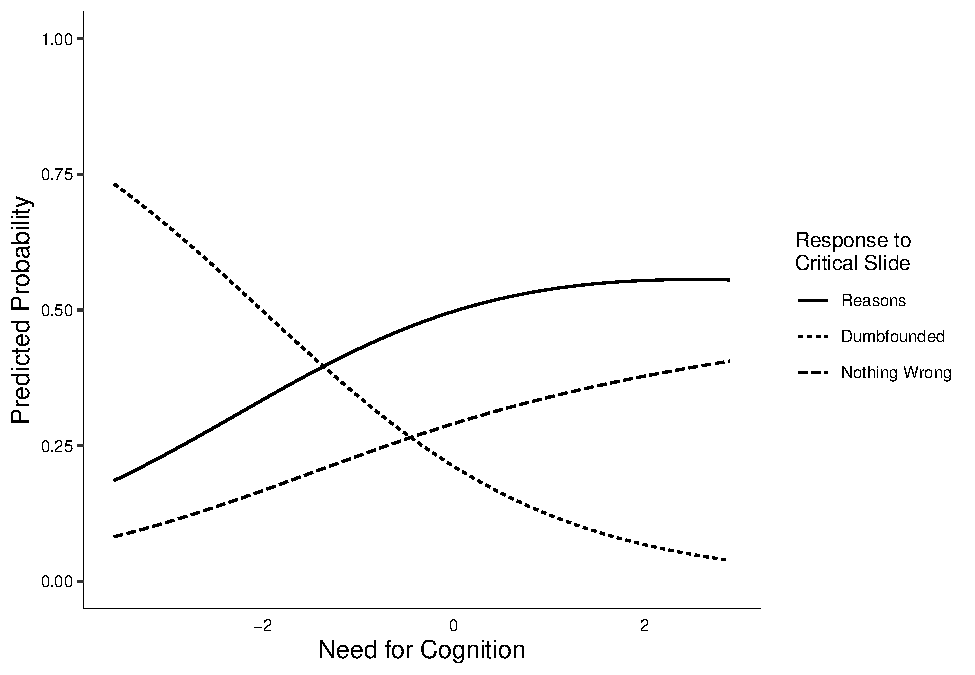
\includegraphics{Supplementary_figures_files/figure-latex/figggplotlogit1-1.pdf}
\caption{\label{fig:figggplotlogit1}Study 1: Probability of selecting each response to the critical slide depending on Need for Cognition}
\end{figure}

\begin{figure}
\centering
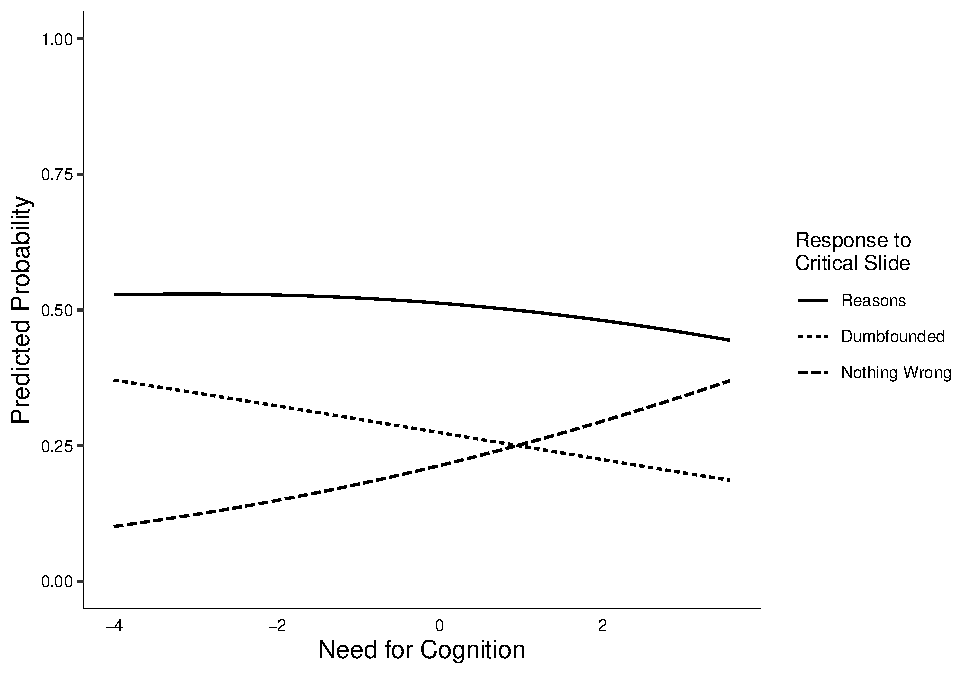
\includegraphics{Supplementary_figures_files/figure-latex/figS2ggplotlogit1-1.pdf}
\caption{\label{fig:figS2ggplotlogit1}Study 2: Probability of selecting each response to the critical slide depending on Need for Cognition}
\end{figure}

\begin{figure}
\centering
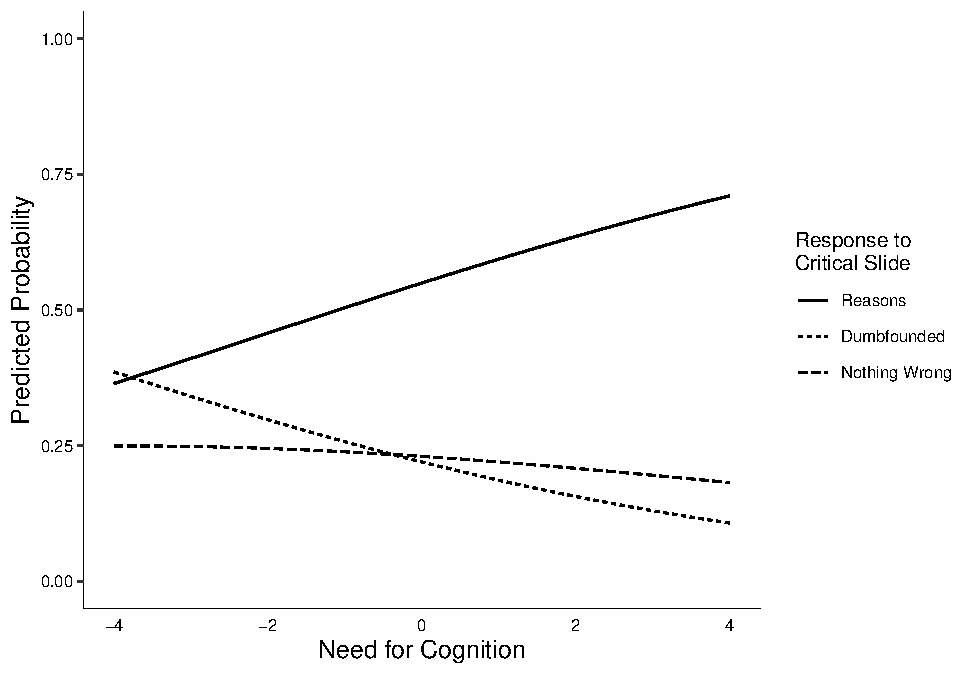
\includegraphics{Supplementary_figures_files/figure-latex/figS3ggplotlogit1-1.pdf}
\caption{\label{fig:figS3ggplotlogit1}Study 3: Probability of selecting each response to the critical slide depending on Need for Cognition}
\end{figure}

\begin{figure}
\centering
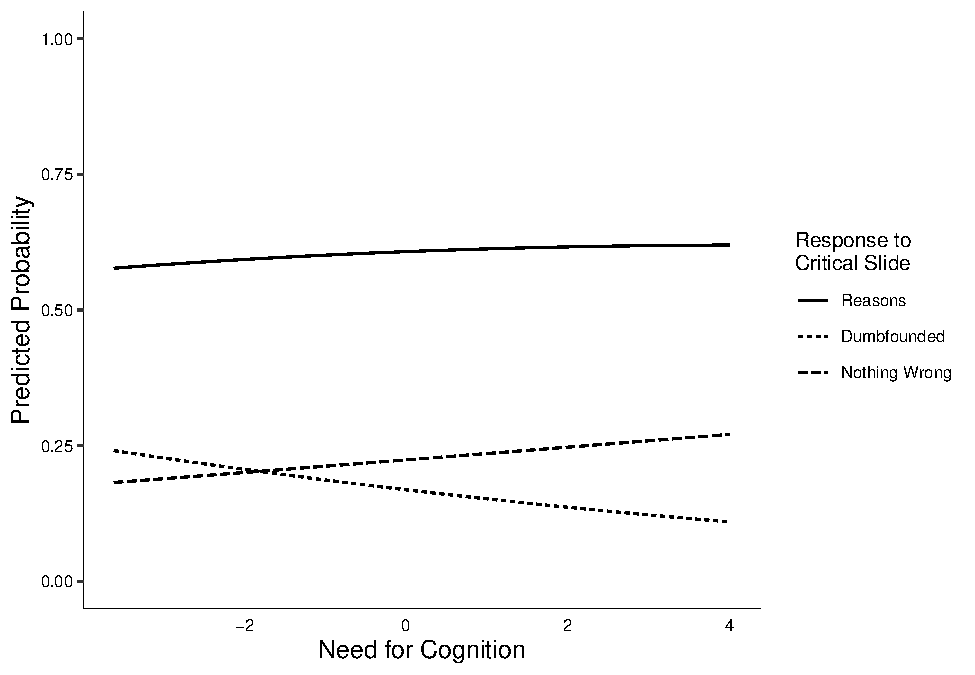
\includegraphics{Supplementary_figures_files/figure-latex/figS4ggplotlogit1-1.pdf}
\caption{\label{fig:figS4ggplotlogit1}Study 4: Probability of selecting each response to the critical slide depending on Need for Cognition}
\end{figure}

\begin{figure}
\centering
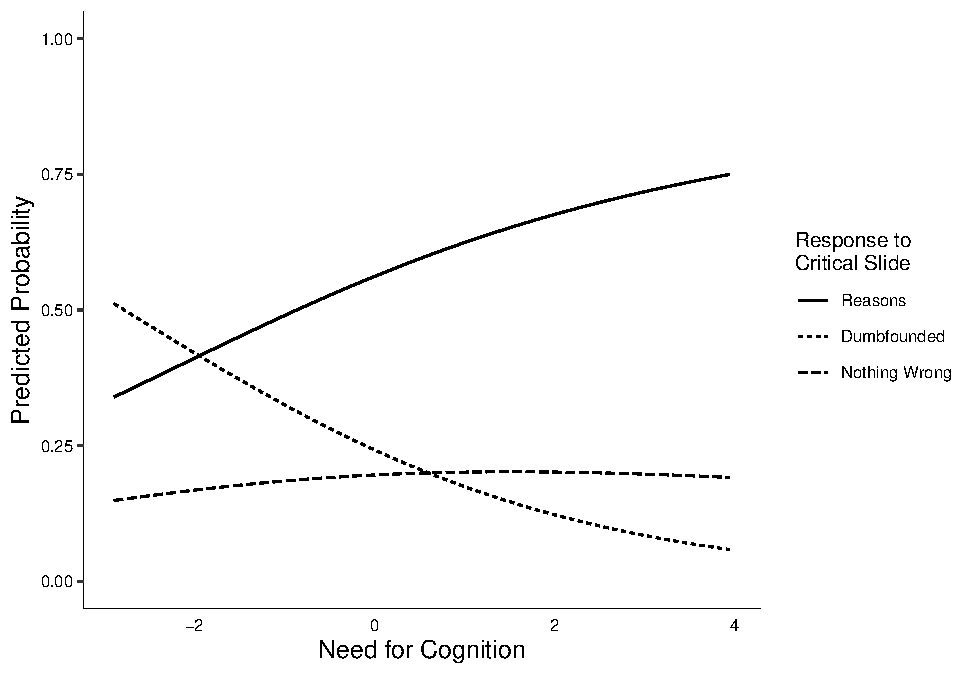
\includegraphics{Supplementary_figures_files/figure-latex/figS5ggplotlogit1-1.pdf}
\caption{\label{fig:figS5ggplotlogit1}Study 5: Probability of selecting each response to the critical slide depending on Need for Cognition}
\end{figure}

\begin{figure}
\centering
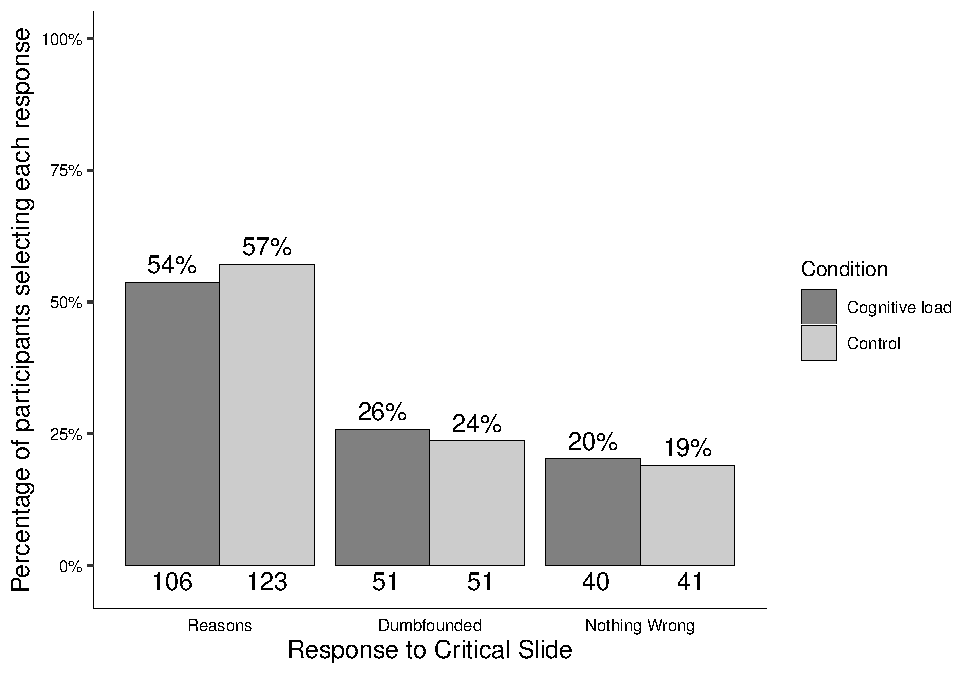
\includegraphics{Supplementary_figures_files/figure-latex/figS6ch5S6fig2criticalconditionbIncest-1.pdf}
\caption{\label{fig:figS6ch5S6fig2criticalconditionbIncest}Study 6: Responses to critical slide depending on cognitive load (Julie and Mark)}
\end{figure}

\begin{figure}
\centering
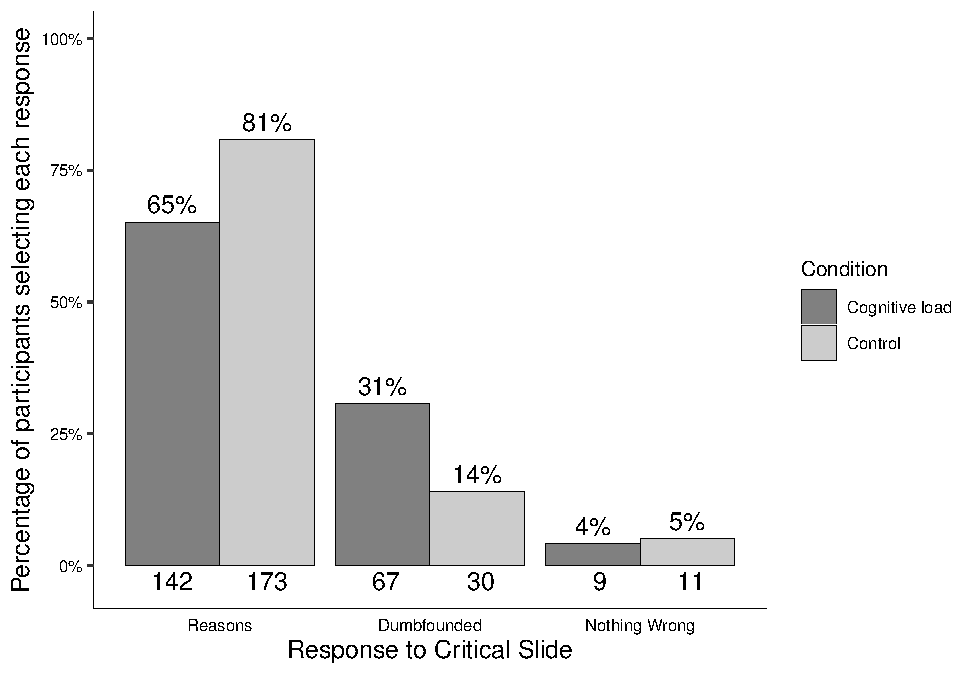
\includegraphics{Supplementary_figures_files/figure-latex/figS6ch5S6fig2criticalconditionbJennifer-1.pdf}
\caption{\label{fig:figS6ch5S6fig2criticalconditionbJennifer}Study 6: Responses to critical slide depending on cognitive load (Jennifer)}
\end{figure}

\begin{figure}
\centering
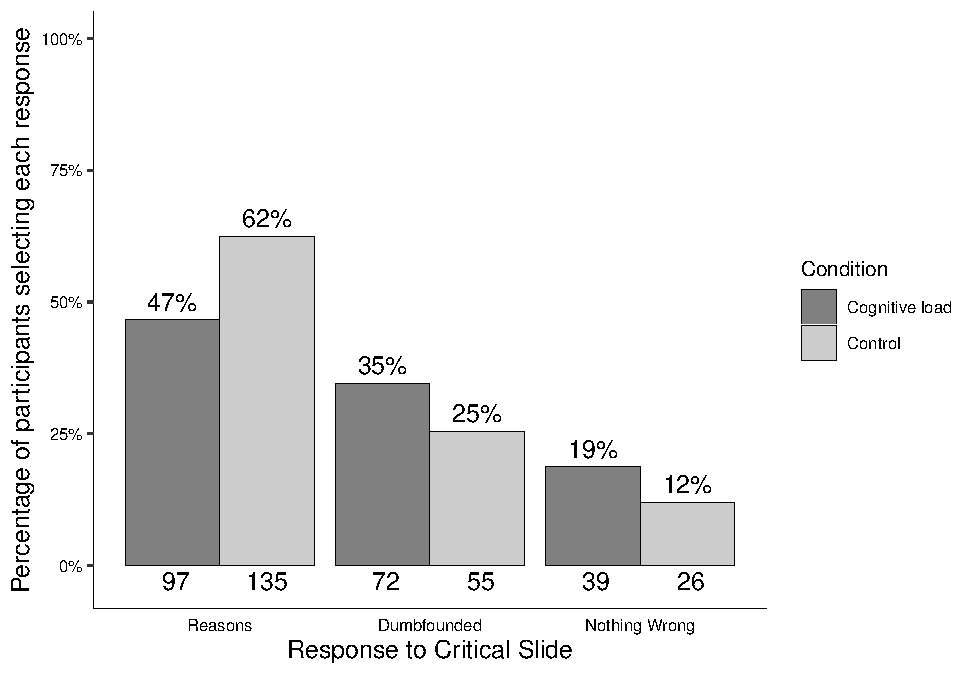
\includegraphics{Supplementary_figures_files/figure-latex/figS6ch5S6fig2criticalconditionbTrolley-1.pdf}
\caption{\label{fig:figS6ch5S6fig2criticalconditionbTrolley}Study 6: Responses to critical slide depending on cognitive load (Trolley)}
\end{figure}

\begin{figure}
\centering
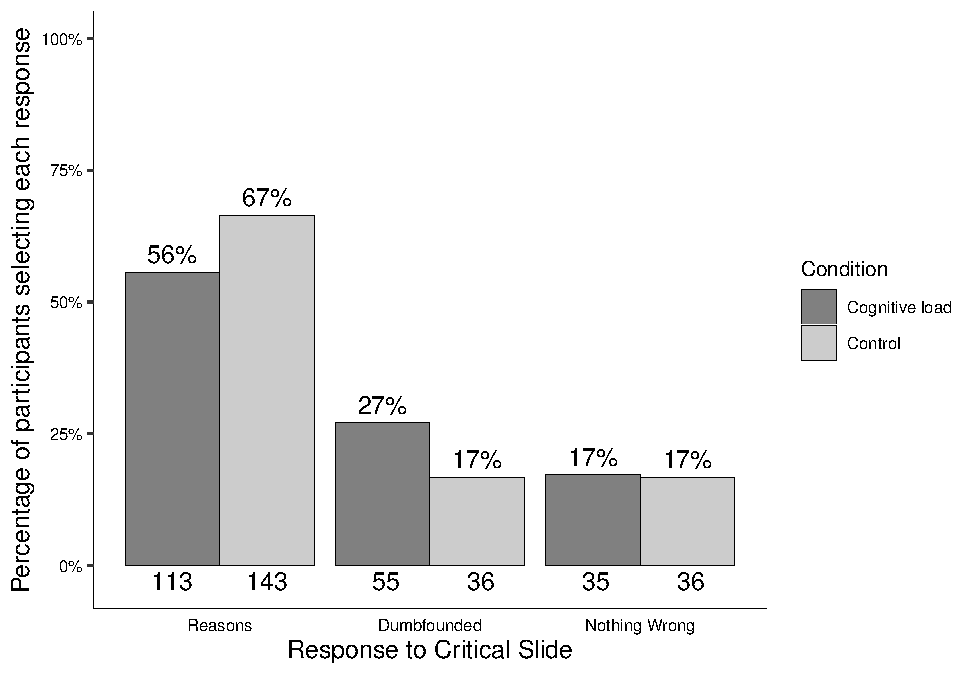
\includegraphics{Supplementary_figures_files/figure-latex/figS6ch5S6fig2criticalconditionbHeinz-1.pdf}
\caption{\label{fig:figS6ch5S6fig2criticalconditionbHeinz}Study 6: Responses to critical slide depending on cognitive load (Heinz)}
\end{figure}


\end{document}
